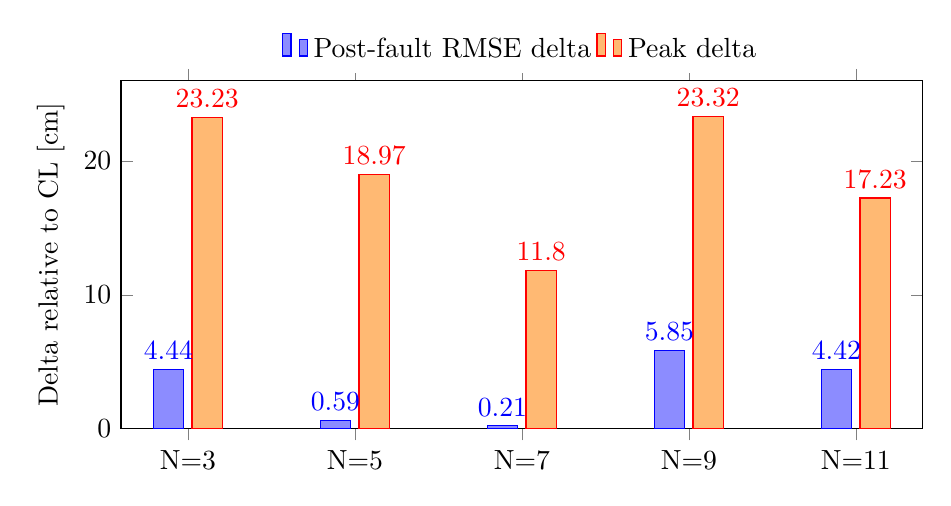
\begin{tikzpicture}
\begin{axis}[
  width=0.97\linewidth,
  height=6.0cm,
  ybar=3pt,
  bar width=11pt,
  ymin=0,
  ymax=26,
  ylabel={Delta relative to CL [cm]},
  symbolic x coords={N=3,N=5,N=7,N=9,N=11},
  xtick=data,
  legend style={at={(0.5,1.02)}, anchor=south, legend columns=2, draw=none},
  nodes near coords,
  nodes near coords align={vertical}
]
\addplot+[fill=blue!45] coordinates {(N=3,4.44) (N=5,0.59) (N=7,0.21) (N=9,5.85) (N=11,4.42)};
\addplot+[fill=orange!55] coordinates {(N=3,23.23) (N=5,18.97) (N=7,11.80) (N=9,23.32) (N=11,17.23)};
\legend{Post-fault RMSE delta,Peak delta}
\end{axis}
\end{tikzpicture}